\documentclass[border=10pt]{standalone}
\usepackage{tikz}
\begin{document}
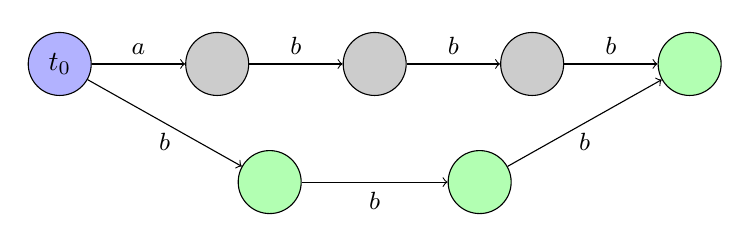
\begin{tikzpicture}[->,sibling distance=10em,
    every node/.style = {shape=circle, rounded corners,
    draw, align=center,minimum size=0.8cm, fill=black!20},
    cgreen/.style={fill=green!30},
    cblue/.style={fill=blue!30}]]
    \node[cblue] (1) at (0, 0) {$t_0$};
    \node (2) at (2, 0) {};
    \node (3) at (4, 0) {};
    \node (4) at (6, 0) {};
    \node[cgreen] (5) at (8, 0) {};
    \node[cgreen] (6) at (2.6666, -1.5) {};
    \node[cgreen] (7) at (5.3333, -1.5) {};
    \path[every node/.style={font=\sffamily\small}]
        (1) edge node[above] {$a$} (2)
        (2) edge node[above] {$b$} (3)
        (3) edge node[above] {$b$} (4)
        (4) edge node[above] {$b$} (5)
        (1) edge node[below] {$b$} (6)
        (6) edge node[below] {$b$} (7)
        (7) edge node[below] {$b$} (5);
\end{tikzpicture}
\end{document}
